\documentclass[conference,compsoc]{IEEEtran}
\usepackage[T1]{fontenc}
\usepackage[utf8]{inputenc}
\usepackage{booktabs,tabularx,array,graphicx,amsmath,amssymb}
\usepackage{placeins}
\usepackage[dvipsnames,table]{xcolor}
\usepackage{tikz}
\usetikzlibrary{arrows.meta,positioning,fit}
\usepackage{pgfplots}
\usepgfplotslibrary{groupplots}
\pgfplotsset{compat=1.18}
\usepackage[hyphens]{url}
\usepackage{hyperref}
\hypersetup{hidelinks,pdfauthor={}}
% Avoid synthetic glyphs at math/text boundaries; preserve Unicode mappings.
\SetSymbolFont{letters}{normal}{OML}{lmm}{m}{it}
\SetSymbolFont{letters}{bold}{OML}{lmm}{b}{it}
\input{glyphtounicode}
\pdfgentounicode=1
\pdfglyphtounicode{space}{0020}
\ifdefined\pdfinterwordspaceoff\pdfinterwordspaceoff\fi
\newcolumntype{Y}{>{\raggedright\arraybackslash}X}
\newcolumntype{P}[1]{>{\raggedright\arraybackslash}p{#1}}
% Replace with the anonymized artifact URL before submission.
\newcommand{\artifacturl}{[anonymized artifact link]}
\newcommand{\papername}{SoK: Agent Communication Side Channels\\Executed Cover and Joint Privacy--State Evaluation}
\title{\papername}
\author{}
\begin{document}
% Shared citation numbering for main paper and supplement.
\nocite{agentprint2025,jeong2026wra,dangol2026workflow,pouryousef2026traffic,song2026personafingerprint,kang2026whoseagent,fayolle2026webagents,shahriar2026agenttell,li2026ant,ayzenshteyn2025cheat,earlybird2025,whisperleak2025,timewilltell2024,wu2026cacheprune,juarez2014critical,mathews2023critical,wang2017walkietalkie,gong2020front,tramer2020adaptive,weiss2024prompt,carlini2024timing,ahmed2023voice,mcp2025transports,rfc9113,rfc8446,uitraces2026,roh2026spillage,chen2010web,chapman2011blackbox,reynolds2006wap5,tak2009vpath,dyer2012peekaboo,trimananda2020pingpong,apthorpe2019stp}

\nocite{duan2026privacytrace,yao2026intentminer}
\nocite{sirinam2018df,bhat2019varcnn,rfc9114,rfc9000}
\nocite{song2026redefining,zavrak2026content}

\nocite{guan2021bapm,deng2023ares,wang2016realistic,hayes2016kfp}

\nocite{zhao2026agenttrace,ediga2026trace,borysenko2026http,borysenko2026short,reworr2024honeypot}

\nocite{arp2022dos}

\nocite{yao2024survey,shahriar2025survey,ferrag2025survey}
\nocite{langchain2025langgraph}

\nocite{debenedetti2025camel,costa2025fides,shi2025progent,yao2024taubench,debenedetti2024agentdojo}
\nocite{cai2014tamaraw}

\raggedbottom
\pagestyle{plain}
\maketitle
\thispagestyle{plain}
\begin{abstract}
When an adversary observes the last hop to a third-party tool, or is the tool, privacy cover cannot be discarded before it reaches the service: decoys must execute as real calls. Their traffic, original-task outcome, business state and resource use must therefore be evaluated together. This early SoK systematizes fifteen Agent communication-side-channel studies (forty-four settings) against twenty-two traffic-analysis anchors and classifies cover by where it terminates, what state it touches, whether its feedback reaches the planner and what process dispatches it. In the four query/workflow privacy settings that exist so far, no setting reports both an adapted attacker and original-task utility under the same intervention. We turn this gap into a joint evaluation contract and apply it to 3,000 single-host executions with two fixed-weight planners over MCP and TLS~1.3/HTTP/2. Controller cover that skips the model wait is removable: given call boundaries, label-free timing removal raises recognition from 75 to 112 (Qwen) and from 80 to 108 (Llama) of 120 tasks. History-matched dispatch removes that shortcut, yet adapted attacks still recognize 93--106/120, a significant gain over size-only attacks in three of four model/arm cells. Without call boundaries, the prespecified removal does not beat its baseline. Against a single shadow planner, the strongest tested attack reaches but does not exceed the 7/12 pair-ambiguity floor of that design, at about twice the model tokens; lowering the floor requires more shadows and proportionally more model work.
\end{abstract}

\section{Introduction}
An Agent receives a support ticket, checks an order and submits a refund through a third-party commerce service. An egress monitor sees which services are contacted, encrypted message sizes and the gaps between requests. A defender who wants to hide the refund adds decoy calls. Classical transport cover would discard those decoys at a cooperating tunnel endpoint~\cite{apthorpe2019stp}, but the commerce service is not under the defender's control and offers no such endpoint. A relay could move the discard point, yet the hop from the relay to the service stays visible to whoever watches it, and the service itself sees every request. Against such observers the decoys must arrive as real requests and execute. Each one now produces two outputs: an observable communication trace and work performed by the application, which may consume quota, touch other objects or enter the planner's context. Evaluating the trace alone leaves the second output unmeasured.

\begin{figure*}[t]
\centering
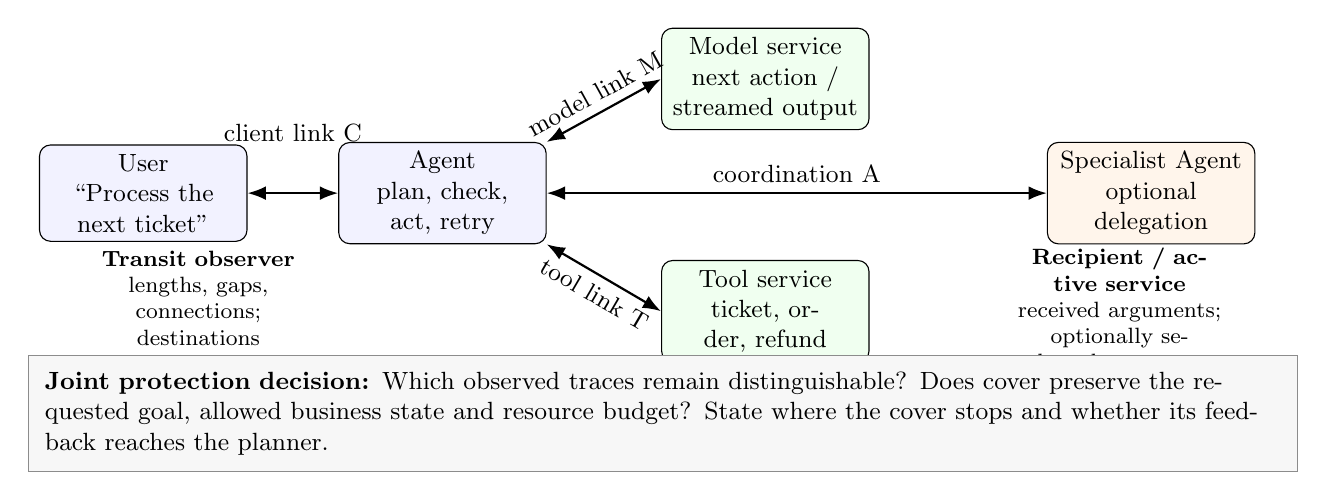
\begin{tikzpicture}[x=1cm,y=1cm,font=\small,>=Latex]
\tikzset{box/.style={draw,rounded corners,align=center,minimum height=.85cm,text width=2.4cm},
 note/.style={align=center,font=\footnotesize,text width=3.1cm}}
\node[box,fill=blue!5] (u) at (1.3,1.15) {User\\``Process the next ticket''};
\node[box,fill=blue!5] (a) at (5.1,1.15) {Agent\\plan, check, act, retry};
\node[box,fill=green!6] (m) at (9.2,2.6) {Model service\\next action / streamed output};
\node[box,fill=green!6] (t) at (9.2,-.35) {Tool service\\ticket, order, refund};
\node[box,fill=orange!8] (d) at (14.1,1.15) {Specialist Agent\\optional delegation};
\draw[<->,thick] (u)--node[above,yshift=15pt]{client link C}(a);
\draw[<->,thick] (a.north east)--node[above,sloped]{model link M}(m.west);
\draw[<->,thick] (a.south east)--node[below,sloped]{tool link T}(t.west);
\draw[<->,thick] (a.east)--node[above]{coordination A}(d.west);
\node[note] at (2.0,-.35) {\textbf{Transit observer}\\lengths, gaps, connections;\\destinations when available};
\node[note] at (13.7,-.35) {\textbf{Recipient / active service}\\received arguments;\\optionally selected responses};
\node[draw=black!45,fill=black!3,align=left,text width=15.7cm,inner sep=6pt] at (7.9,-1.65) {
\textbf{Joint protection decision:} Which observed traces remain distinguishable? Does cover preserve the requested goal, allowed business state and resource budget? State where the cover stops and whether its feedback reaches the planner.};
\end{tikzpicture}
\caption{Running support-ticket example and observation rights. A tool result returns to the Agent and can enter the next model request. Each encrypted link exposes its own traffic shape; a recipient additionally sees the request addressed to it. Concurrent tickets may share a connection on either link. The arrows represent application communication, not a one-to-one mapping from tool events to packets.}
\label{fig:chain}
\end{figure*}


\paragraph{The research question}
How should Agent communication defenses be evaluated when cover is executable work? Agent side-channel research is young: our bounded retrieval finds fifteen direct studies, most of them preprints. This early SoK therefore does not estimate field-wide frequencies. It fixes the evaluation object before practice settles: it classifies cover by its termination point, state access, feedback visibility and dispatcher, states when cover must execute (Section~\ref{sec:taxonomy}), maps all forty-four existing settings onto that object, and tests the resulting contract on live executions.

\textbf{A privacy result needs outcomes from the same protected execution.} WRA's published research decoys reduce query recovery from .770 to .565, while its report-utility scores 8.55 and 8.54 belong to a different intervention that changes destination visibility~\cite{jeong2026wra}. The communication-graph study refits an attacker on protected OHTTP captures and reports traffic cost, but not original-task utility under that intervention~\cite{dangol2026workflow}. In the four query/workflow privacy settings that exist so far, none reports both.

\textbf{The process generating cover is itself observable.} Honest tool calls follow model decisions; a naive controller can insert cover without that wait. We use such immediate cover as a calibration baseline: given call boundaries, label-free gap removal restores recognition to 112/120 and 108/120. The substantive tests concern history-matched dispatch, which removes the shortcut but still leaves 93--106/120 recognition under adapted attacks, and a complete shadow planner, whose strongest tested attack sits at the 7/12 pair-ambiguity floor that one independent shadow permits. Task, state and costs are measured on the same runs.

WF and ML-security work already requires realistic observation units, protected-condition attacks and matched costs~\cite{juarez2014critical,mathews2023critical,arp2022dos,tramer2020adaptive}. Agent execution adds three requirements: say where cover terminates, what it may change and whether its results return to the planner.

\paragraph{Contributions}
\begin{itemize}
\item \textbf{A cover taxonomy and necessity rule} (Section~\ref{sec:taxonomy}): cover policies classified by termination, state, feedback and dispatcher, with the deployment conditions under which cover must execute.
\item \textbf{An execution-aware field map and joint contract} (Sections~\ref{sec:correspondence}--\ref{sec:defenses}, \ref{sec:reporting}): all forty-four settings, their transfer relations, and a checklist that binds residual inference, task completion, business invariants and resource cost to one intervention.
\item \textbf{A live test of the contract} (Section~\ref{sec:experiment}): controller dispatch is removable, history matching is not sufficient, and the strongest tested attack on planner cover is explained by a pair-ambiguity floor; we derive how that floor and the model work scale with the number of shadows.
\end{itemize}

\section{Scope and Evidence Construction}\label{sec:scope}
The evidence map connects Agent execution to an observed communication signal, a hidden target and the rights needed to observe it.

\subsection{Inclusion and retrieval}
An Agent uses an LLM to select actions, with external feedback able to affect later action or termination. Client, tool, model and inter-agent interfaces are eligible. Transit observers obtain traffic metadata; contacted recipients see their addressed requests; active auditors also choose probes or challenges. Negative results qualify: PrivacyTrace's metadata/order condition remains included despite scoring below its prior reference~\cite{duan2026privacytrace}. Whole semantic trajectories or browser instrumentation alone enter the adjacent layer, while deliberate covert messages and prompt-injection defenses without communication-side inference remain contextual related work~\cite{yao2026intentminer,uitraces2026}.

The fixed eligibility window covers first public submissions from 1 January 2024 through 9 November 2026. Twelve topic queries, a native arXiv query and inclusion rules preceded the retrieval pass; title/publication checks and one-step citation follow-ups completed it. The arXiv query returned 180 records. Public-web queries supplied 33 scholarly candidates across 101 displayed URLs; deduplication yielded 209 records. Two citation leads brought screening to 211: fourteen direct, forty adjacent, 155 outside scope and two unresolved identities. The eligible CHeaT (Cloak, Honey, Trap) seed adds the fifteenth direct source (Figure~\ref{fig:selection-main}). The SSH honeypot entered through citation tracing, illustrating the value of combining retrieval routes. Exact queries and dispositions are in the supplement.
\begin{figure}[t]\centering
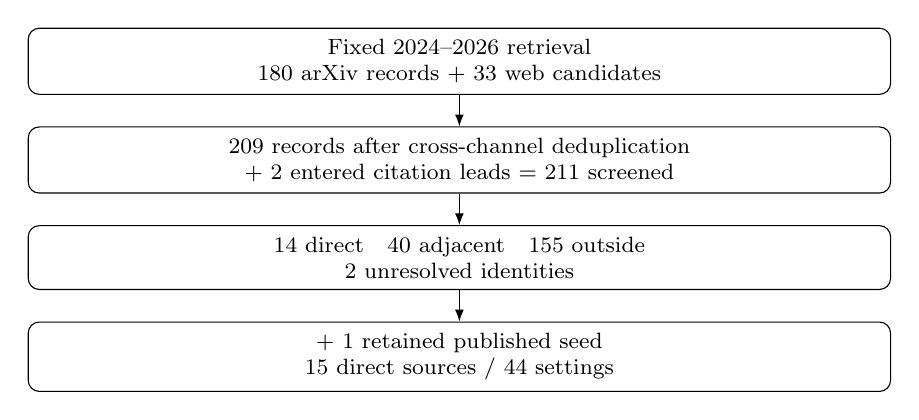
\begin{tikzpicture}[node distance=4mm,box/.style={draw,rounded corners,align=center,text width=.88\columnwidth,inner sep=4pt,font=\footnotesize},arr/.style={-{Latex[length=1.5mm]}}]
\node[box] (a) {Fixed 2024--2026 retrieval\\180 arXiv records + 33 web candidates};
\node[box,below=of a] (b) {209 records after cross-channel deduplication\\+ 2 entered citation leads = 211 screened};
\node[box,below=of b] (c) {14 direct\quad40 adjacent\quad155 outside\\2 unresolved identities};
\node[box,below=of c] (d) {+ 1 retained published seed\\15 direct sources / 44 settings};
\draw[arr] (a)--(b);\draw[arr] (b)--(c);\draw[arr] (c)--(d);
\end{tikzpicture}
\caption{Executed coverage audit. Counts are deduplicated work/lead records; two identities remain unresolved. Mechanism anchors use a separate inclusion rule.}
\label{fig:selection-main}
\end{figure}


Twenty-two separately selected mechanism anchors comprise sixteen published communication studies and six serving studies. They supply the established relations in the transfer matrix; the fifteen direct studies supply the Agent application evidence. These layers retain separate inclusion records and denominators. The anchor set is selected for mechanism correspondence, rather than a census of classical traffic analysis.

\subsection{Extraction and source dependencies}
Forty-four setting records bind source version and locator to access, features, learner, target, population, split, intervention, result and cost. Labels, execution outcomes, failure treatment and policy context are recorded alongside them. WRA and CHeaT are checked against official USENIX texts. One HTTP study has a verified ACM workshop identity, while its detailed measurements come from the extended arXiv version~\cite{borysenko2026http,borysenko2026short}. Twelve other works lack independently verified formal publication identities at the cutoff.

Text reading, displayed-number reconstruction, selected-code inspection and data recomputation have separate entries in the extraction sheet. For example, WRA's decoy and visibility conditions are checked in the published text; OHTTP refitting is checked in selected code. Each check supports its matched premise. Section~\ref{sec:sensitivity} reports what remains when sources are removed. The author assigned and decided every code against the cited passage. AI tools located candidate passages and proposed draft codes, which the author accepted, changed or rejected. Two further AI passes audited the codebook; they are not inter-rater reliability. An independent security PhD researcher, blind to the manuscript and author codes, re-coded the decision-critical subset from the sources. Access class (44/44), intervention purpose (9/9), and adaptation and utility in the four privacy settings (4/4 each) agree fully ($\kappa=1$). The protection flag agrees on 38/44 ($\kappa=.61$) and transfer relations on 5/6 ($\kappa=.77$); after source adjudication of the seven disagreements, no setting has both an adapted attacker and matched utility (Supplement S6.1). The source-located table in Supplement S7 lists each privacy decision. The low-agreement execution-outcome field enters only the descriptive coverage summary in Supplement S6.

For the descriptive summary, every setting receives an access class and intervention purpose. Protected-condition adaptation and original-task utility are counted within the four query/workflow privacy settings. Three identity-obfuscation and two adversarial-Agent blocking settings have different objectives; one composition setting re-measures CG-transform's protections and is counted with it; thirty-four settings contain no protection comparison. A located item identifies evidence in the retained record. An unlocated item leaves that question open. The supplementary reporting ledger lists the assignments and source locators.

\subsection{Relation to security surveys and Agent defenses}
Broader surveys organize LLM and Agent threats by lifecycle, attack surface and defensive role~\cite{yao2024survey,shahriar2025survey,ferrag2025survey}. This SoK asks three communication-specific questions: which service representation reaches which observer, whether an intervention covers the later feedback path, and what business work its cover can trigger. The maps connect each answer to a measured setting and its evidence strength. The supplementary deployment section compares these surveys and WF systematizations.

Information-flow and privilege controls address closely related execution boundaries. CaMeL tracks dependencies and explicitly discusses tool-call and timing side channels~\cite{debenedetti2025camel}; FIDES enforces confidentiality/integrity policies and selectively exposes tool information~\cite{costa2025fides}; Progent constrains tool calls and arguments~\cite{shi2025progent}. SPILLage distinguishes content and behavioral oversharing by browser Agents~\cite{roh2026spillage}. Our maps add the communication-observer question: which metadata remain visible under a particular deployment and intervention? They do not replace these policy mechanisms. Likewise, $\tau$-bench and AgentDojo already evaluate environment outcomes~\cite{yao2024taubench,debenedetti2024agentdojo}. The cover example applies state-aware evaluation to matched traffic measurements; state checking itself is established practice.

\section{Threat Model and Classification}\label{sec:taxonomy}
\textbf{A result is meaningful only for the target and observations actually supplied to its attacker.}
The ticket example has client--Agent, Agent--model, Agent--tool and coordination links (Figure~\ref{fig:chain}). A transit observer sees connection destinations, directions, lengths and times. A contacted service reads the request addressed to it; an active auditor can also choose challenges. Table~\ref{tab:deployment-access} maps these rights to deployment configurations. The same traffic may encode requested intent, a logged action or successful execution. Authorization additionally requires the principal and policy context: identifying a refund does not decide whether it was approved.

\begin{table*}[t]\centering\small
\caption{Deployment and access map. The configurations are analyst-defined; cited settings test the listed view, not every component of the deployment. A gateway's plaintext access requires TLS termination.}\label{tab:deployment-access}
\setlength{\tabcolsep}{4pt}
\begin{tabularx}{\textwidth}{@{}P{.18\textwidth}P{.25\textwidth}P{.28\textwidth}Y@{}}\toprule
Deployment & Observer and permitted view & Existing evidence for that view & Protection consequence \\\midrule
Enterprise egress & A transit monitor sees routed model/tool flows, sizes, times and any exposed destination association. & WRA: supplied research-domain traces; ANT and cloud benchmark: model/combined traffic~\cite{jeong2026wra,li2026ant,pouryousef2026traffic}. & Specify which services cross the monitored egress. A union of flows is available only when the monitor can observe them. \\\addlinespace[3pt]
Shared gateway or relay & Transit sees multiplexed gateway output. A terminating gateway can additionally read addressed requests. & Live OHTTP: passive-link inference under stated relay trust~\cite{dangol2026workflow}; PrivacyTrace: semantic recipient/gateway access~\cite{duan2026privacytrace}. & Separate relay association protection from content trust. Connection sharing changes the observation unit. \\\addlinespace[3pt]
Local model, remote tools & An external observer sees remote tool traffic; the local model call has no corresponding external network leg. & WRA's destination-recovery mechanism is relevant to tool egress~\cite{jeong2026wra}; whole-deployment protection is untested in the mapped comparison. & Evaluate tool and downstream calls. Do not import a remote-model attack score into an absent network leg. \\\addlinespace[3pt]
Cloud model, remote tools & An authorized vantage may see either or both encrypted legs. A contacted tool sees its own arguments. & ANT/cloud benchmark test model traffic~\cite{li2026ant,pouryousef2026traffic}; PrivacyTrace tests recipient-visible representations~\cite{duan2026privacytrace}. & Check permitted model and tool views after the intervention; recipients and passive monitors need different protections. \\\bottomrule
\end{tabularx}
\end{table*}


\subsection{What is observed and what is predicted}
A captured packet, TLS record, HTTP stream, tool call and complete task are different units. A gateway can regroup streamed output; HTTP/2 and QUIC can multiplex streams; MCP may use local stdio or remote HTTP~\cite{mcp2025transports,rfc9113,rfc9114,rfc9000,rfc8446}. A boundary supplied by the evaluator is prior information, not a classifier output. Six fields specify each inference setting: interface and representation, observer access, supplied prior information, prediction target, evaluation population and base rate, and protected-training access. Host traces can supply experimental truth without becoming transit-visible features~\cite{reynolds2006wap5,tak2009vpath}.

\subsection{When cover must execute}\label{sec:necessity}
Transport cover ends before a business tool, at an endpoint the defender controls~\cite{apthorpe2019stp}. That endpoint must sit after the observer: otherwise the observer can see it discard the cover. A defender can sometimes move the endpoint, for example to a relay outside a monitored egress, but the segment from the last defender-controlled hop to the service remains. If the adversary can observe that segment, or is the service itself, every request it sees must be real. Cover then hides a real call only by arriving as a real call (Table~\ref{tab:cover-necessity}). Executed cover therefore follows from the deployment; it is not a design preference. It crosses an application boundary: it may consume quota, access other objects, update state or enter the planner's context.

\begin{table}[t]\centering\footnotesize
\caption{When cover must execute. Transport cover needs a defender-controlled terminator located after the observer and before the business service. Without one, cover can hide the real call only by arriving as a real call.}\label{tab:cover-necessity}
\setlength{\tabcolsep}{3pt}
\begin{tabularx}{\columnwidth}{@{}P{.27\columnwidth}P{.2\columnwidth}Y@{}}\toprule
Observer $\to$ service & Terminator after observer? & Cover that can work \\\midrule
Egress $\to$ own service & Yes (own tunnel) & Transport cover suffices~\cite{apthorpe2019stp} \\\addlinespace[2pt]
Egress $\to$ third-party SaaS or remote MCP & No & Executed cover; isolation only if the provider offers it \\\addlinespace[2pt]
Recipient (tool provider) & No & Executed cover whose arguments must also be plausible to the recipient \\\addlinespace[2pt]
TLS-terminating gateway & After gateway only & Executed cover, or trust the gateway with content \\\bottomrule
\end{tabularx}\end{table}


\subsection{A taxonomy of cover}\label{sec:cover-taxonomy}
We classify a cover policy along four axes (Table~\ref{tab:cover-taxonomy}). \emph{Termination and state} determine what business work cover performs. \emph{Feedback visibility} determines whether cover responses enter later model requests. The \emph{dispatcher}, the process that decides when cover is sent, determines whether cover inherits the timing of honest calls. Honest calls follow a model decision; a controller that inserts cover without waiting for the model creates a timing signature that has no counterpart in the first three axes. The live study varies the dispatcher while holding termination (an isolated clone) and feedback (hidden) fixed.

\begin{table*}[t]\centering\small
\caption{Cover taxonomy. Each policy is classified by where it terminates and what state it touches, whether its responses reach the real planner, and which process dispatches it. The last column names the evaluation in which the policy is measured; S1 is the earlier state control and Section~\ref{sec:cover-study} the live timing study.}\label{tab:cover-taxonomy}
\setlength{\tabcolsep}{4pt}
\begin{tabularx}{\textwidth}{@{}P{.17\textwidth}P{.26\textwidth}P{.13\textwidth}P{.2\textwidth}Y@{}}\toprule
Policy & Terminates at / state touched & Feedback to planner & Dispatcher & Measured in \\\midrule
Transport cover & Tunnel endpoint before the service; no business state & No & Sender schedule & STP~\cite{apthorpe2019stp}; WF padding~\cite{juarez2016wtfpad,gong2020front} \\
Proxy discard & Defender proxy computes on a disposable copy & No & Controller & S1 \\
Read cover & Real service; reads only & No & Controller & S1 \\
Isolated execution & Real service on a persistent clone & No / yes & Controller & S1 (hidden and visible); all live cover arms \\
Live write & Real service on production state & No & Controller & S1 (stress control) \\
Research decoys & Real third-party Web destinations & Not located & Decoy generator & WRA~\cite{jeong2026wra} \\\midrule
Immediate & Isolated clone & No & Controller, directly after an honest response & Section~\ref{sec:cover-study} (calibration) \\
History-matched & Isolated clone & No & Controller, training-gap and duration samples; sequential or concurrent & Section~\ref{sec:cover-study} \\
Planner shadow & Isolated clone; separate planner context & No & Second planner on an independent ticket & Section~\ref{sec:cover-study} \\\bottomrule
\end{tabularx}\end{table*}


The live study models the second row of Table~\ref{tab:cover-necessity} when the observed hop is the last one before the service: seven MCP services stand for third-party tools, no defender relay intervenes, and the observer is a transit monitor on that path. Information forwarded to another service creates another permitted observation; it does not imply that every service is visible to the same attacker. The recipient view of executed cover, where the attacker also reads decoy arguments, is not evaluated here and remains open (Section~\ref{sec:agenda}).

\section{Evidence Map and Classical Conditions}\label{sec:correspondence}
\textbf{Most mapped settings evaluate recognition; only four settings from two sources support the selected query/workflow privacy comparisons.}
Tables~\ref{tab:complete-matrix-a}--\ref{tab:complete-matrix-b} display all forty-four settings. They preserve the source-defined target and unit rather than rank incompatible accuracy, reconstruction and prevention scores. Twenty-two settings use transit observations, ten use recipient access, eleven active access, and one inferred preferences. Three settings compare identity obfuscation and two compare adversarial-Agent blocking; these are separate from user/workflow privacy.

\begin{table*}[t]\centering\footnotesize
\caption{Complete setting matrix, part 1 of 2. Each row is one of the forty-four retained settings. Scores keep the source's metric and target; they are not cross-paper rankings. Access states the observer's rights. Last column gives intervention purpose and, for the four privacy comparisons, adapted attack / same-intervention original-task utility (yes or NR: not located). A dash is outside that denominator. Shared* is counted with CG-transform. Full features, split rules and locators remain in the extraction sheet.}\label{tab:complete-matrix-a}
\setlength{\tabcolsep}{3pt}\renewcommand{\arraystretch}{1.12}
\begin{tabularx}{\textwidth}{@{}P{.14\textwidth}P{.11\textwidth}P{.13\textwidth}P{.14\textwidth}P{.12\textwidth}Y P{.09\textwidth}@{}}\toprule
Work / setting & Link; access & Target & Signal / learner & Evaluation unit & Source result & Purpose; A/U \\\midrule

AP-identity~\cite{agentprint2025} & client; transit & hosted-agent identity & Packet size/direction; CNN & interaction & F1 .8660 closed; .8477 open & none; -- \\
AP-behavior~\cite{agentprint2025} & client; transit & interaction mode & Packet size/direction; CNN & interaction & F1 .924/.889 conflict & none; -- \\
AP-persona~\cite{agentprint2025} & preferences; derived & occupation & Inferred preferences & participant preferences & Top-3 occupation 69.1\% & none; -- \\
WRA-prompt~\cite{jeong2026wra} & tool/Web; transit & prompt meaning & Domains/time; LLM & research task & Query recovery .770 / .725 & none; -- \\
WRA-persona~\cite{jeong2026wra} & tool/Web; transit & user traits & Domains/time; LLM & multiple sessions & Separate trait-category scores & none; -- \\
WRA-decoy~\cite{jeong2026wra} & tool/Web; transit & prompt meaning & Domains/time; LLM & research task & .770 to .565; five decoys & privacy; NR/NR \\
WRA-visibility~\cite{jeong2026wra} & tool/Web; transit & prompt meaning & Domains/time; LLM & research task & .770/.610; quality 8.55/8.54 & privacy; NR/yes \\
CG-workflow~\cite{dangol2026workflow} & coord.; transit & workflow class & Graph/size/time; RF & workflow & Nine-class accuracy .67 & none; -- \\
CG-composition~\cite{dangol2026workflow} & coord.; transit & workflow class & Graph/size/time; RF & workflow & Known-label holdout .18 & shared*; -- \\
CG-MCP~\cite{dangol2026workflow} & tool; transit & sequence class & Graph/size/time; RF & fixed sequence & Fixed-sequence accuracy .99 & none; -- \\
CG-transform~\cite{dangol2026workflow} & coord.; transit & workflow class & Graph/size/time; RF & workflow & Capture transformation; separate from live & privacy; yes/NR \\
CG-live~\cite{dangol2026workflow} & coord.; transit & workflow class & Graph/size/time; RF & workflow & Six-class .30; 13x bytes, 11x delay & privacy; yes/NR \\
CG-active~\cite{dangol2026workflow} & coord.; active & integrity impact & Graph/size/time; RF & pending workflow & Live integrity endpoint & none; -- \\
CB-task~\cite{pouryousef2026traffic} & model; transit & task & Traffic statistics; RF & MARBLE execution & Ten-class BA .853/.860 & none; -- \\
CB-topology~\cite{pouryousef2026traffic} & model; transit & task & Traffic statistics; RF & execution & Topology change .83 to .52 & none; -- \\
CB-size-excluded~\cite{pouryousef2026traffic} & model; transit & task class & Traffic statistics; RF & execution & BA .540/.587 & none; -- \\
CB-partial~\cite{pouryousef2026traffic} & model; transit & task & Traffic statistics; RF & execution & One-agent BA .665/.780 & none; -- \\
PF-session~\cite{song2026personafingerprint} & tool/Web; transit & synthetic persona & Signed intervals; CNN & fixed packet window & Per-site persona F1 .78--.91 & none; -- \\
PF-pooled~\cite{song2026personafingerprint} & tool/Web; transit & synthetic persona & Signed intervals; CNN & packet window & Pooled summaries conflict & none; -- \\
PF-open~\cite{song2026personafingerprint} & tool/Web; transit & persona membership & Signed intervals; CNN & window & Open-world misattribution & none; -- \\
MARK-protocol~\cite{kang2026whoseagent} & tool/Web; recipient & agent stack identity & Protocol/headers & trial & TLS/H2 F1 .725; HTTP .799 & none; -- \\
MARK-combined~\cite{kang2026whoseagent} & tool/Web; recipient & agent identity & Protocol/headers & trial & Combined F1 .971 & none; -- \\
\bottomrule\end{tabularx}\end{table*}

\begin{table*}[t]\centering\footnotesize
\caption{Complete setting matrix, part 2 of 2. Each row is one of the forty-four retained settings. Scores keep the source's metric and target; they are not cross-paper rankings. Access states the observer's rights. Last column gives intervention purpose and, for the four privacy comparisons, adapted attack / same-intervention original-task utility (yes or NR: not located). A dash is outside that denominator. Shared* is counted with CG-transform. Full features, split rules and locators remain in the extraction sheet.}\label{tab:complete-matrix-b}
\setlength{\tabcolsep}{3pt}\renewcommand{\arraystretch}{1.12}
\begin{tabularx}{\textwidth}{@{}P{.14\textwidth}P{.11\textwidth}P{.13\textwidth}P{.14\textwidth}P{.12\textwidth}Y P{.09\textwidth}@{}}\toprule
Work / setting & Link; access & Target & Signal / learner & Evaluation unit & Source result & Purpose; A/U \\\midrule

FAY-network~\cite{fayolle2026webagents} & tool/Web; recipient & implementation & Protocol/site features & connection/request & Layer-specific distinguishability & identity; -- \\
FAY-combined~\cite{fayolle2026webagents} & tool/Web; recipient & agent identity & Protocol/site features & visit & Combined fingerprint view & identity; -- \\
FAY-blocking~\cite{fayolle2026webagents} & tool/Web; active & access outcome & Protocol/site features & visit & Access success; not privacy score & blocking; -- \\
AT-choice~\cite{shahriar2026agenttell} & tool/Web; active & cross-origin fact & Challenge choice & two-origin session & 61.1\% loaded choice; cold-adjusted LS & none; -- \\
ANT-scenario~\cite{li2026ant} & egress; transit & scenario & Direction/size/time & episode & Five-task accuracy .431--.727 & none; -- \\
ANT-model-scope~\cite{li2026ant} & model/rest; transit & scenario & Direction/size/time & episode & Eight approximate model-view scores & none; -- \\
ANT-risk~\cite{li2026ant} & egress; transit & benchmark risk label & Direction/size/time & episode & 209 episodes; risk recall .15--.95 & none; -- \\
ANT-stage~\cite{li2026ant} & egress; transit & primitive group & Direction/size/time & primitive segment & 47-group accuracy .355--.462 & none; -- \\
CHT-lure~\cite{ayzenshteyn2025cheat} & asset; active & LLM-based visitor presence & Lure/output/challenge & probe interaction & Presence mechanism; no natural F1 & none; -- \\
CHT-password~\cite{ayzenshteyn2025cheat} & output; active & LLM presence & Lure/output/challenge & challenge response & Password-output control & none; -- \\
CHT-blocking~\cite{ayzenshteyn2025cheat} & CTF; active & defender prevention success & Lure/output/challenge & CTF attempt & CTF prevention endpoint & blocking; -- \\
PT-metadata~\cite{duan2026privacytrace} & tool; recipient & profile attributes & Tool metadata/arguments & single-domain trajectory & ASR .1453; prior .1797 & none; -- \\
PT-content~\cite{duan2026privacytrace} & tool; recipient & profile attributes & Tool metadata/arguments & single-domain trajectory & Arguments ASR .2771 & none; -- \\
ATR-main~\cite{zhao2026agenttrace} & tool; active & model identity & Arguments/repairs & multi-probe attribution trial & 50-probe accuracy .960 & none; -- \\
ATR-budget~\cite{zhao2026agenttrace} & tool; active & model identity & Arguments/repairs & multi-probe attribution trial & 1--50 probes: .652--.960 & none; -- \\
ATR-obfuscation~\cite{zhao2026agenttrace} & tool; active & model identity & Arguments/repairs & multi-probe attribution trial & Attribution above .94 & identity; -- \\
TR-within~\cite{ediga2026trace} & terminal; recipient & model family & Terminal n-grams; SVM & terminal session & Mixed-session F1 .981 & none; -- \\
TR-scaffold~\cite{ediga2026trace} & terminal; recipient & model family & Terminal n-grams; SVM & terminal session & Scaffold holdout F1 .815 & none; -- \\
TR-proprietary~\cite{ediga2026trace} & terminal; recipient & model family & Terminal n-grams; SVM & terminal session & Accuracy .78; narrower models & none; -- \\
HTTP-signature~\cite{borysenko2026http} & docs; recipient & implementation & HTTP trace & documentation-retrieval trial & 9 agents/6 services; descriptive & none; -- \\
HP-calibration~\cite{reworr2024honeypot} & SSH; active & Agent candidate & Timing/prompt responses & controlled probe interaction & Probe timing about 1.7s & none; -- \\
HP-field~\cite{reworr2024honeypot} & SSH; active & Agent candidate & Timing/prompt responses & field interaction/session & 8 candidates; identity unverified & none; -- \\
\bottomrule\end{tabularx}\end{table*}


\subsection{What transfers from communication analysis}
Table~\ref{tab:transfer-matrix} separates established evaluation conditions from additional Agent execution conditions. WF already addresses open-world populations, base rates, unknown boundaries and adaptive attacks~\cite{juarez2014critical,wang2016realistic,guan2021bapm,deng2023ares,mathews2023critical}. Web and IoT work connects action-dependent messages to observable events~\cite{chen2010web,chapman2011blackbox,trimananda2020pingpong,ahmed2023voice}. Agent execution couples those events to model waits, tool state and later feedback. A condition is retained when it applies directly, extended when an execution condition must be added, and untested when the mapped Agent evidence does not evaluate the corresponding claim. These are relationships, not maturity levels.

\begin{table*}[t]\centering\small
\caption{Transfer of established conditions to Agent execution. Relationship labels concern the stated mapping; evidence strength and missing tests appear separately. A missing Agent test does not refute the classical result.}\label{tab:transfer-matrix}
\setlength{\tabcolsep}{4pt}
\begin{tabularx}{\textwidth}{@{}P{.25\textwidth}P{.29\textwidth}P{.10\textwidth}Y@{}}\toprule
Established relation and condition & Agent mapping / consequence & Relation & Agent evidence and remaining test \\\midrule
Unknown boundaries and background affect event recognition~\cite{wang2016realistic,guan2021bapm,deng2023ares,trimananda2020pingpong}. & Tool bursts, model waits and task intervals are different units. Evaluate proposed events with false alarms as well as classification. & Extended & ANT supplies stage boundaries; the local concurrent study tests particular detectors. Greater Agent localization difficulty is untested. \\\addlinespace[3pt]
Defense evaluation must allow adaptation to the protected distribution~\cite{dyer2012peekaboo,mathews2023critical,tramer2020adaptive}. & Record protected training access and still-visible links; an unchanged learner family can refit. & Retained & Transformed and live OHTTP settings report adaptation in one preprint~\cite{dangol2026workflow}; WRA's matched protected examples remain unresolved. \\\addlinespace[3pt]
Coarse timing/volume can remain useful under specified padding~\cite{dyer2012peekaboo}; serving streams expose length/gap signals~\cite{weiss2024prompt,whisperleak2025}. & Name the shaping policy, receiving hop and Agent workload before carrying over a measured effect. & Untested generalization & Cloud and ANT measure model-view recognition~\cite{pouryousef2026traffic,li2026ant}. A general protected-Agent SSE claim is not tested by these observations. \\\addlinespace[3pt]
An observation result is tied to the visible paths and representations~\cite{chen2010web,apthorpe2019stp}. & Feedback forwards tool information into later model requests across separately controlled services; evaluate every permitted residual view. & Extended & Published WRA tool-side evidence and preprint model/recipient results establish different exposed interfaces. Causal feedback attribution needs its own test. \\\addlinespace[3pt]
STP tunnel endpoints remove cover before it reaches devices or servers~\cite[Sec.~7.1]{apthorpe2019stp}. & When cover executes as research, add original-task resource, state and feedback constraints to the traffic budget. & Extended & Published WRA reports executed research decoys and utility under a different intervention~\cite{jeong2026wra}. Our controlled LLM case separates task completion from state integrity (Section~\ref{sec:cover-study}); it does not evaluate WRA writes. \\\addlinespace[3pt]
Host traces can reconstruct distributed request paths~\cite{reynolds2006wap5,tak2009vpath}. & Instrumentation can provide ground truth; a transit attacker must infer from its own permitted observations. & Access mismatch & ANT stage labels and local task intervals are evaluator-provided. Host tracing alone cannot establish passive encrypted-stream localization. \\\bottomrule
\end{tabularx}
\end{table*}


\subsection{Changes of execution are distinct tests}
Communication-graph composition holdout keeps nine known labels and changes their capability combinations: reported accuracy moves from about .67 to .18~\cite{dangol2026workflow}. A cloud benchmark's graph/star comparison instead changes coordination, with about .83 to .52 under its matched feature protocol~\cite{pouryousef2026traffic}. Trace holds out Agent scaffolds for model-family attribution, reporting macro-F1 .815 versus .981 in a mixed-session test~\cite{ediga2026trace}. These are version-specific observations on different targets. A pooled transfer score would erase the condition each tests. Failures also select the population: first-pass attribution, repaired trajectories and successful-run filtering answer different questions.

\section{Executed Cover Changes the Evaluation Contract}\label{sec:evidence}
\textbf{A deployable cover policy must meet both its inference target and the business constraints of the original task.}
The map supplies two practical distinctions: evidence from different interventions cannot be joined into a single operating point, and original-task completion covers only part of application utility.

\subsection{Protection and utility must name the same intervention}\label{sec:targets}
WRA's five research decoys lower functional query recovery from .770 to .565. Its 8.55/8.54 report-utility comparison instead changes destination visibility from 100\% to 10\%, with recovery .770/.610~\cite{jeong2026wra}. Those utility scores do not price the executed-decoy result. This distinction blocks a concrete interpretation: the pair cannot establish that five decoys preserve report quality at that measured level.

The communication-graph live OHTTP setting reports six-class accuracy .30, approximately thirteen-fold bytes and eleven-fold latency, with protected-capture RF refitting~\cite{dangol2026workflow}. Its nine-class .67 workflow result is a different population. Traffic cost is recorded, while original-task utility under that intervention remains unresolved. Table~\ref{tab:availability} gives each eligible setting and its evidence. Among four settings, adaptation is documented in two and matched task utility in one; no setting documents both. The count identifies a gap in these inspected configurations.

\subsection{Business state is separate from goal completion}\label{sec:authorization}
A goal predicate can hold while another order, shared quota or ledger is wrong. A joint record therefore separates requested-goal success, violations of declared business invariants, and resource use. In production, invariants should allow legitimate concurrent updates; exact state equality is appropriate for a fixture whose intended transition is fully specified. State-aware evaluation already exists in $\tau$-bench and AgentDojo~\cite{yao2024taubench,debenedetti2024agentdojo}. Our contribution connects it to the same traffic-protection intervention and adapted observations.

An execution contract names the allowed objects and transitions, quota/token budgets and feedback that cover may expose to the real planner. Isolation prevents direct cover writes to production state but still consumes compute and can change scheduling. A response being hidden from the planner does not undo the underlying operation. Section~\ref{sec:cover-study} evaluates these outputs separately.

\subsection{Protection scope includes other permitted views}\label{sec:crosslink}
WRA observes research destinations, whereas ANT and the cloud benchmark measure tasks on model connections~\cite{jeong2026wra,li2026ant,pouryousef2026traffic}. A recipient additionally sees its addressed arguments: PrivacyTrace reports attribute-inference ASR .2771 with arguments, versus .1453 for metadata/order and a .1797 schema reference~\cite{duan2026privacytrace}. This is an access distinction, not a ranking across attackers. Forwarded tool results enter later model requests, alongside initial task fields and model decisions. A tool-only defense must therefore state which other views its attacker retains.

\section{Defense Mechanisms and Execution Costs}\label{sec:defenses}
\textbf{The layer that controls a signal determines which protection and business costs it can change.}
Table~\ref{tab:defense-space} classifies naming, representation, scheduling, transport cover, execution cover and shared-state isolation. The map extends traffic-budget comparisons with tool privileges, business state and model work.

\begin{table*}[t]\centering\small
\caption{Defense design space: enforcement authority, costs to measure and remaining exposure. Source-specific measurements appear in the text and Supplement S7.}
\label{tab:defense-space}
\setlength{\tabcolsep}{4pt}
\begin{tabularx}{\textwidth}{@{}P{.17\textwidth}P{.25\textwidth}P{.23\textwidth}Y@{}}\toprule
Layer / mechanism & What must be trusted or controlled & Costs to measure together & Residual exposure and practical decision \\\midrule
Naming / association: encrypted name resolution, relays, OHTTP & Name resolver or relay placement; the parties able to link the user to the destination & Added hops, bytes, latency and availability & Shape can survive name hiding. Choose this layer when destination association is the private target; then test remaining observers. \\\addlinespace[3pt]
Representation: message, TLS-record or packet padding & Component that controls the final visible size; padding survives later encoding & Added bytes, record/packet count, fragmentation & Timing, count and other links remain. State the padding layer and test downstream captures. \\\addlinespace[3pt]
Scheduling: batching, pacing, fixed-rate cover & Sender/relay controls output schedule and cover lifetime & First-response delay, completion delay, bandwidth during idle periods & Admission, termination and overflow can reveal activity. Budget these events as part of the visible trace. \\\addlinespace[3pt]
Transport cover: dummy exchanges discarded at a tunnel endpoint & Trusted cover terminator; no dispatch into business tools & Cover bandwidth, queueing, resource use & Other endpoints still see their inputs. Prefer this boundary when the aim is traffic shaping without extra business work. \\\addlinespace[3pt]
Execution cover: extra research or tool calls & Tool privileges, isolated state and whether decoy feedback reaches the planner & Model tokens, tool quota, task success, state changes and latency & A decoy can affect the real execution. Measure privacy and original-task utility on the same protected runs. \\\addlinespace[3pt]
Shared-state isolation / minimization & Tenant separation, cache keys and information passed between services & Lost cache reuse, compute, latency, task accuracy & Isolation removes a sharing channel, not every traffic signal. Minimize tool arguments and feedback according to each recipient's role. \\\bottomrule
\end{tabularx}
\end{table*}


Name hiding changes destination association; message padding changes lengths; pacing changes timing and termination. STP's tunnel endpoints discard cover before devices process it~\cite{apthorpe2019stp}. Walkie-Talkie, FRONT, Adaptive Padding and WTF-PAD supply different scheduling and overhead choices~\cite{wang2017walkietalkie,gong2020front,shmatikov2006adaptive,juarez2016wtfpad}. Their evaluation lessons carry over, while executed research or tool calls add application work. Matching interarrival marginals alone is not a new security principle: receive-dependent padding already models request--response dependencies. The Agent-specific object tested here is the controller/model decision process that generates tool calls.

Model services introduce additional timing and sharing signals. Token streams, cache behavior and token count can remain observable under particular interfaces~\cite{weiss2024prompt,whisperleak2025,earlybird2025,timewilltell2024,carlini2024timing,wu2026cacheprune}. A tool-message padding rule does not determine a later model request's shape. Defense comparisons should report the achieved downstream trace, task/state outcomes and resources together.

\section{A Joint Evaluation of Executed Cover}\label{sec:experiment}
\textbf{The dispatcher changes residual inference and resource use; business correctness needs its own endpoint.}
Table~\ref{tab:study-map} lists the populations used here. Each keeps its own denominators, and only the families named there are primary.

\begin{table}[t]\centering\footnotesize
\caption{Study map. Each population answers one question and keeps its own denominators and statistical role.}\label{tab:study-map}
\setlength{\tabcolsep}{3pt}
\begin{tabularx}{\columnwidth}{@{}P{.2\columnwidth}P{.25\columnwidth}Y@{}}\toprule
Study & Population; observer & Question; role \\\midrule
Live timing (\S\ref{sec:cover-study}) & 3,000 episodes + 600 shadow chains; call windows, TLS record times & Does the dispatcher expose cover? Primary families P, R, C \\\addlinespace[2pt]
Record-only (\S\ref{sec:no-call}) & Same episodes; no call boundaries & How much survives without supplied boundaries? Retrospective; one primary pair \\\addlinespace[2pt]
State control (\S\ref{sec:business}; S1) & 3,600 episodes; call windows, sizes only & Does goal completion miss collateral state? Primary state family \\\addlinespace[2pt]
Forwarding pilot (S10) & 3,120 local + 192 hosted & Feedback attribution; inconclusive, supplement only \\\bottomrule
\end{tabularx}\end{table}


\paragraph{Statistical conventions}
These apply throughout this section and are not repeated. \emph{Sel.}\ is the attack chosen on validation data before test scoring; primary tests use only these choices. \emph{Max} is the largest test count in a finite attack suite; it is descriptive and is not an upper bound on inference. \emph{Exploratory} marks an analysis designed after test results were seen. Intervals condition on the fitted attacks and the designed workload. All runs are on one host over loopback with synthetic tools and fixtures reused across studies; Section~\ref{sec:validity} lists what this does not test.

\begin{figure}[t]\centering
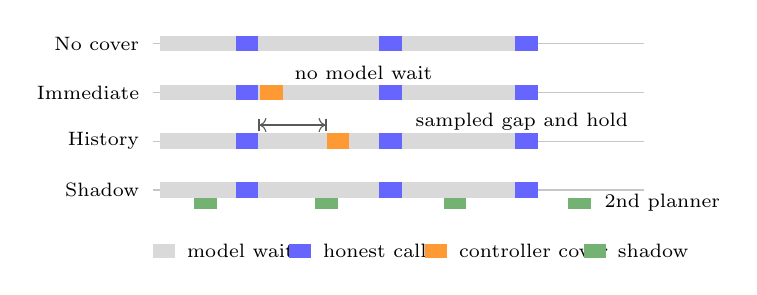
\begin{tikzpicture}[x=.48cm,y=.62cm,font=\scriptsize]
\def\bar#1#2#3#4{\fill[#4] (#1,#3-.16) rectangle (#2,#3+.16);}
\foreach \y/\n in {4/No cover,3/Immediate,2/History,1/Shadow}{
 \node[anchor=east] at (-.1,\y) {\n};
 \draw[gray!45] (0,\y)--(13,\y);
 \bar{0.2}{2.2}{\y}{gray!30}\bar{2.2}{2.8}{\y}{blue!60}
 \bar{2.8}{6.0}{\y}{gray!30}\bar{6.0}{6.6}{\y}{blue!60}
 \bar{6.6}{9.6}{\y}{gray!30}\bar{9.6}{10.2}{\y}{blue!60}}
% immediate cover: right after the honest response
\bar{2.85}{3.45}{3}{orange!80}
\node[anchor=west] at (3.5,3.4) {no model wait};
% history cover: after a sampled gap
\bar{4.6}{5.2}{2}{orange!80}
\draw[|<->|,gray!70!black] (2.8,2.33)--(4.6,2.33);
\node[anchor=west] at (6.7,2.4) {sampled gap and hold};
% shadow chain: its own model waits
\foreach \a in {1.1,4.3,7.7,11.0}{\fill[green!45!black!55] (\a,.62) rectangle (\a+.6,.84);}
\node[anchor=west] at (11.7,.73) {2nd planner};
% legend
\begin{scope}[yshift=-.25cm]
\fill[gray!30] (0,0) rectangle (.6,.3); \node[anchor=west] at (.65,.15) {model wait};
\fill[blue!60] (3.6,0) rectangle (4.2,.3); \node[anchor=west] at (4.25,.15) {honest call};
\fill[orange!80] (7.2,0) rectangle (7.8,.3); \node[anchor=west] at (7.85,.15) {controller cover};
\fill[green!45!black!55] (11.4,0) rectangle (12.0,.3); \node[anchor=west] at (12.05,.15) {shadow};
\end{scope}
\end{tikzpicture}
\caption{Dispatchers in the live study. Honest calls follow a model wait. Immediate cover follows the previous response without one, which label-free gap removal exploits. History-matched cover samples a training gap and response hold. Shadow calls come from a second planner, so their gaps are model waits too.}\label{fig:dispatch}
\end{figure}

\subsection{Actual dispatch and timing-aware attacks}\label{sec:cover-study}
\textbf{Cover inherits the timing of whatever process dispatches it.}
Two fixed-weight planners, Qwen3:8B and Llama3.1:8B, each execute 300 fixtures in five conditions, yielding 3,000 main episodes and 600 additional shadow chains. The six business actions use seven MCP services through LangGraph over TLS~1.3/HTTP/2; the services stand for third-party tools that offer no cover terminator (Table~\ref{tab:cover-necessity}). Partitions contain 120 training, 60 validation and 120 paired test fixtures per cell. The task label is requested intent; failures remain included. Cover executes on an isolated clone and its responses are hidden from the real planner.

The four cover arms vary only the dispatcher (Figure~\ref{fig:dispatch}). \emph{Immediate} cover follows an honest response directly. \emph{History} cover samples a training-only honest gap and service duration, waits in real time and holds the response for the sampled minimum; the \emph{sequential} variant blocks the real chain, the \emph{concurrent} one overlaps real model inference. \emph{Shadow} runs a complete second planner on an independent, uniformly drawn ticket; a fair draw decides which chain starts first. Calls to the same service serialize. The observer receives destinations, ciphertext bytes, TLS record completion times and supplied episode/call windows; Section~\ref{sec:no-call} withdraws the call windows.

\begin{table*}[t]\centering\small
\caption{Joint evaluation of the five live policies; 120 test fixtures per row, single host over loopback, synthetic tools. Sel.\ S/A: validation-selected size-only / adaptive attack (primary). Max: largest test count in the frozen suite (descriptive). GMM: label-free removal. Ref.: uniform six-class reference 20/120, or for shadow the realized pair-ambiguity floor (Table~\ref{tab:shadow-floor}). Bytes: whole-connection / call-window factors. Tokens include both planners. Goal and State are separate counts from this cohort; the state-control cohort (Supplement S1) has its own counts.}\label{tab:live-timing-main}
\setlength{\tabcolsep}{4pt}
\begin{tabularx}{\textwidth}{@{}lYrrrrrrr@{}}\toprule
Planner & Policy & Sel. S/A & Max & GMM & Ref. & Bytes$\times$ & Tokens$\times$ & Goal/State \\\midrule

Qwen3:8B & No cover & 117/117 & 117 & -- & 20 & 1.00/1.00 & 1.00 & 113/114 \\
Qwen3:8B & Immediate & 75/112 & 112 & 112 & 20 & 1.15/1.33 & 1.00 & 111/112 \\
Qwen3:8B & History, sequential & 76/93 & 99 & 53 & 20 & 1.15/1.32 & 1.00 & 112/113 \\
Qwen3:8B & History, concurrent & 66/99 & 99 & 38 & 20 & 1.15/1.33 & 1.00 & 111/112 \\
Qwen3:8B & Planner shadow & 54/54 & 70 & 34 & 70.5 & 1.31/1.68 & 2.01 & 112/113 \\
Llama3.1:8B & No cover & 110/110 & 112 & -- & 20 & 1.00/1.00 & 1.00 & 82/70 \\
Llama3.1:8B & Immediate & 80/108 & 108 & 108 & 20 & 1.13/1.27 & 1.01 & 83/67 \\
Llama3.1:8B & History, sequential & 82/104 & 104 & 14 & 20 & 1.13/1.26 & 1.01 & 84/67 \\
Llama3.1:8B & History, concurrent & 68/106 & 106 & 66 & 20 & 1.13/1.27 & 1.02 & 82/67 \\
Llama3.1:8B & Planner shadow & 64/64 & 64 & 43 & 70.5 & 1.35/1.71 & 1.99 & 82/67 \\
\bottomrule\end{tabularx}\end{table*}


\paragraph{Immediate cover: a calibration baseline}
A label-free two-component mixture over training gaps selects the short-gap component for removal; a classifier trained on no-cover traffic decodes the rest. This restores 112/120 and 108/120 correct predictions, against selected non-timing attacks at 75 and 80, and meets the prespecified replication rule in both models after Holm correction. The result confirms the mechanism rather than reporting a new weakness: a controller that skips the model wait is removable. Independent TCP reassembly matches all 773,450 recorded TLS record types, lengths and counts, and refitting the mixture on packet-capture clocks reproduces both scores (Supplement S2).

\paragraph{History matching removes the shortcut, not the signal}
History sampling defeats the simple mixture, but adapted context removal or joint decoding still recognizes 93/120 and 104/120 sequential executions, against selected non-timing attacks at 76 and 82 (Holm $p=.0559$ and $.00078$). Concurrent dispatch gives 99/120 and 106/120 against 66 and 68; both 27.5- and 31.7-point advantages pass correction. The policy controls minimum waits, not achieved timing: Qwen's mean sampled hold of 40.5\,ms becomes 100.4\,ms sequential and 171.2\,ms concurrent at the record observer. A failed simple attack is therefore not evidence of concealment. Llama's sequential mixture deletes 477/634 honest calls while detecting only 64/182 cover calls, which explains its 14/120, while adapted joint decoding on the same traces reaches 104/120.

\begin{table}[t]\centering\footnotesize
\caption{Pair-ambiguity floor $P^*(k)$ for $k$ shadow planners and six classes, computed exactly (\texttt{experiment/shadow\_floor.py}). \emph{iid}: shadow labels drawn uniformly; \emph{distinct}: drawn without replacement from classes other than the real one. Tokens are nominal planner multiples. Only $k=1$, iid, was run.}\label{tab:shadow-floor}
\setlength{\tabcolsep}{4pt}
\begin{tabular}{@{}rrrrl@{}}\toprule
$k$ & iid & distinct & Tokens$\times$ & Live result ($k=1$) \\\midrule
0 & 1.000 & -- & 1 & \\
1 & .583 & .500 & 2 & Max 70 / 64 of 120 \\
2 & .491 & .333 & 3 & \\
3 & .456 & .250 & 4 & \\
4 & .428 & .200 & 5 & \\\midrule
\multicolumn{5}{@{}l}{Realized $k=1$ floor on the test split: 70.5/120 (21 matching labels)} \\\bottomrule
\end{tabular}\end{table}


\paragraph{Planner shadow sits at its pair-ambiguity floor}
Suppose an attacker separates the real chain from $k$ shadow chains perfectly and recovers every chain's label, but cannot tell which chain is real. If the real chain is exchangeable with the shadows, the best guess is the modal label, which succeeds with probability $P^*(k)=\mathbb{E}[\max_c n_c]/(k+1)$ for $n_c$ chains labeled $c$. With one shadow and six uniform classes, $P^*(1)=1/6+\tfrac{5}{6}\cdot\tfrac12=7/12$ (Table~\ref{tab:shadow-floor}). On the realized test split, 21 of 120 shadow labels match the real one, so the floor is 70.5/120.

The strongest tested attack, a size/destination random forest, scores 70/120 for Qwen and 64/120 for Llama; the validation-selected attacks score 54 and 64. Neither exceeds the floor, so the tested attacks are no more accurate than an attacker who already knew both tasks, and the 16.7\% uniform reference is the wrong comparison for this design. The floor is not a bound: real tickets are reused fixtures with their own cache histories, so exchangeability is an idealization, and an attacker who learns role cues could exceed it. A chain-separation attack scores 49 and 34 and recovers the real chain exactly in only 29 and 32 fixtures. Which chain the attacker can identify is a separate question. Among the 99 fixtures whose labels differ, the aggregate counts bound the real-label accuracy of the forest only to $[49,70]/99$ and $[43,64]/99$. An exact role test against 50\% needs the saved per-fixture predictions and is part of the artifact (Section~\ref{sec:validity}). The prespecified equivalence family E is degenerate here, because both selectors chose the same attack and every pair ties; we do not count it as evidence.

Shadow costs 2.01/1.99 times the model tokens, 1.68/1.71 times the call-window bytes, and raises mean real-chain time from 2.91/3.33\,s to 4.80/3.94\,s. Table~\ref{tab:shadow-floor} shows the trade-off this implies: each further independent shadow adds one planner's work and lowers the floor slowly, whereas drawing shadow labels without replacement from the other classes lowers it to $1/(k+1)$ at no extra cost. Neither variant was run; both are the next measurements this design calls for. Supplement S2 retains every attack, test and cost.

\subsection{Recognition without supplied call boundaries}\label{sec:no-call}
\textbf{Without call boundaries, the prespecified removal attack loses its advantage.}
We reanalyze all 3,000 episodes from complete encrypted connections, including initialization and closing records. The attacker receives relative record times, directions, ciphertext lengths and destinations, but no call starts or ends, operation names, role labels or HTTP stream assignment. Whole-episode association remains supplied, so this withdraws call boundaries, not task localization. A per-connection idle-gap rule proposes events, with five gaps from 5 to 250\,ms competing on validation accuracy; raw-record classifiers skip eventization. LR and RF use destination summaries and early/late event sequences, with and without timing, and a training-only mixture removes short-gap events before a no-cover classifier. This is a retrospective, fixed-protocol analysis of reused fixtures; the immediate-arm pair is its only primary test, with Holm over the two models.

\begin{table}[t]\centering\small
\caption{No supplied call boundaries; whole-episode association remains supplied. B/R: validation-selected idle-grid baseline and removal attacks (primary pair: immediate). Max: largest test count over both suites, including the exploratory protocol-aware eventizer designed after the idle-grid results were seen (descriptive). Counts out of 120; uniform reference 20.}\label{tab:no-call-main}
\setlength{\tabcolsep}{4pt}
\begin{tabularx}{\columnwidth}{@{}Yrrrr@{}}\toprule
 & \multicolumn{2}{c}{Qwen} & \multicolumn{2}{c}{Llama} \\\cmidrule(lr){2-3}\cmidrule(l){4-5}
Policy & B/R & Max & B/R & Max \\\midrule
No cover & 115/109 & 117 & 108/101 & 112 \\
Immediate & 80/69 & 91 & 90/86 & 97 \\
History, sequential & 73/74 & 75 & 88/56 & 93 \\
History, concurrent & 56/61 & 62 & 78/62 & 88 \\
Planner shadow & 69/65 & 73 & 69/56 & 69 \\
\bottomrule\end{tabularx}\end{table}

On immediate cover, selected removal recognizes 69/120 and 86/120 tasks, against baselines of 80 and 90: paired differences of $-9.2$ and $-3.3$ points (Holm $p=.025$ and $.54$). Removal is worse than the baseline for Qwen and indistinguishable for Llama, so the call-window removal advantage does not carry over to this pipeline. An exploratory eventizer, designed after these results were seen, uses the public request-padding quantum and MCP setup sequence to mark proposed requests and responses; it reads no call truth. It raises Qwen's removal count from 68 to 91 but lowers Llama's from 90 to 87. Because the representations differ, the gap from the call-window counts is not a pure causal effect of boundaries. Its event recovery is poor: protocol-event F1 is 0.295 and 0.380 at IoU .5 on immediate cover, so task recognition here does not imply recovering calls. For shadow, the Qwen maximum of 73/120 over 52 candidates is 2.5 fixtures above the realized floor; the selected attacks (69 and 69) are below it. Supplement S3 gives the protocol and the event audit.

\subsection{Business constraints and the protection decision}\label{sec:business}
Every live cover arm executes in isolated state and hides cover feedback from the real planner. Table~\ref{tab:live-timing-main} reports goal/state counts on the same fixtures as inference and costs. Shadow outcomes are 112/113 for Qwen and 82/67 for Llama, versus no-cover 113/114 and 82/70. These are different endpoint counts: a correctly preserved state need not contain a successful intended action. Low Llama baseline performance and changed planning paths limit business-equivalence conclusions.

The earlier six-policy study supplies a deliberately adverse state control (Supplement S1). Read/proxy/hidden-isolated cover retains Qwen state correctness at 115--116/120. Live writes can alter other objects and reduce it to 7/120; 95 of 102 completed Qwen tasks have collateral errors. Llama's corresponding counts are 3/120 intact and 73 of 76 completed tasks with collateral errors. The harm direction is built into that stress condition: it tests whether the evaluation records forbidden effects, not how often production writes cause them.

The combined decision is concrete. Immediate cover leaves high inference after removal. Historical dispatch changes that attack but retains substantial adapted inference. Shadow execution trades model work for a trace whose strongest tested attack sits at the design's pair-ambiguity floor; lowering that floor needs more shadows. An adverse write can fail the state contract even when the requested goal passes. Choosing a policy requires stating acceptable inference, task, state and resource tolerances rather than comparing a single accuracy decrease.

\section{A Reusable Joint Evaluation Protocol}\label{sec:reporting}
\textbf{Privacy, task success, business state and cost must refer to the same intervention and evaluation population.}
Table~\ref{tab:joint-checklist} is a compact reporting form; the procedure below explains how to use it. It combines established security-evaluation guidance~\cite{arp2022dos,juarez2014critical,mathews2023critical,tramer2020adaptive} with explicit cover execution constraints. It is a reporting proposal, not a measured analyst-performance improvement.

\begin{table*}[t]\centering\small
\caption{Joint evaluation checklist. Complete all applicable entries for one intervention and population; attach evidence or state the missing item. Goal completion and whole-state correctness have separate fields.}\label{tab:joint-checklist}
\begin{tabularx}{\textwidth}{@{}lYlY@{}}\toprule
 & Entry & & Entry \\\midrule
$\square$ & Hidden target, population, prior/base rate & $\square$ & Allowed observations and supplied boundaries \\
$\square$ & Cover termination, privileges and isolation & $\square$ & Planner-visible cover feedback and dispatcher \\
$\square$ & Adapted attacks and largest tested residual & $\square$ & Original-task attempts, completion and failures \\
$\square$ & Business invariants and violations & $\square$ & Matched bytes, latency, tokens and quota \\\bottomrule
\end{tabularx}\end{table*}

\begin{table*}[t]\centering\small
\caption{Evidence located in the retained records. Counts use eligible settings; the second column also gives distinct sources. ``Not located'' leaves evidence unresolved within the inspected scope. These counts describe availability, not study quality or checklist validity.}\label{tab:availability}
\setlength{\tabcolsep}{4pt}
\begin{tabularx}{\textwidth}{@{}P{.28\textwidth}P{.15\textwidth}P{.11\textwidth}Y@{}}\toprule
Question & Eligible settings / sources & Located & Supporting settings and consequence \\\midrule
Protected-condition attack adaptation & 4 / 2 & 2/4 & Communication graphs: transformed captures and live OHTTP. Both come from one preprint. \\\addlinespace[3pt]
Original-task utility under the same intervention & 4 / 2 & 1/4 & WRA visibility comparison. It does not price WRA's executed-decoy condition. \\\addlinespace[3pt]
Adaptation and original-task utility in one setting & 4 / 2 & 0/4 & Adaptation and utility are located in different records; transport cost alone does not fill the task-outcome field. \\\addlinespace[3pt]
Original-task utility for executed cover & 1 / 1 & 0/1 & WRA's five research decoys report recovery and extra research; matched original-task utility is not located. \\\bottomrule
\end{tabularx}
\end{table*}


\begin{enumerate}
\item \textbf{Specify observations and execution authority.} Name the hidden target, visible links, recipient rights and supplied boundaries. State where cover ends, which state it can access and whether its responses reach the planner.
\item \textbf{Specify business invariants and budgets.} Define the original goal, allowed collateral transitions and quota/token/latency tolerances. Separate a goal that was attempted, one that completed and a whole execution satisfying its state contract.
\item \textbf{Measure matched executions and adapted attacks.} Pair baseline and policy on the same workload. Include cover-detection/removal and schedule-aware attacks, plus the largest tested residual inference. Report original-task outcomes and all resource costs from those protected runs.
\item \textbf{Decide using the declared tolerances.} An execution outside its state or resource contract fails that requirement even if its goal passes. An attacker exceeding the allowed inference threshold defeats the corresponding protection claim. Passing a finite attack suite is not a general secrecy proof.
\end{enumerate}

\paragraph{Source-matched examples}
WRA-decoy fills the privacy and extra-research fields, while its original-task quality under that intervention is unresolved. WRA-visibility supplies matched quality, but for a different policy. Live OHTTP supplies adapted inference and traffic cost, while original-task utility remains unresolved. ANT supplies observation/label evidence without a protection comparison. These entries preserve each study's scope; they are not paper-quality scores. Supplement S7 gives the complete source-located forms.

\section{Synthesis and Research Agenda}\label{sec:agenda}
\textbf{The field map turns a privacy score into a protection decision by binding its observations to executable work.}
The strongest cross-study consequence is intervention matching: WRA's visibility utility cannot establish executed-decoy utility, and adapted OHTTP inference with traffic cost does not establish original-task preservation. The technical case adds the dispatcher: controller cover can omit model waits and become removable, history matching hides the shortcut but not the signal, and planner cover is bounded by a pair-ambiguity floor that only more model work can lower. These connections extend the evaluation object; the underlying adaptive-attack and state-correctness principles are established.

\subsection{Source dependence}\label{sec:sensitivity}
The evidence map follows 33 statements in seven comparisons across 20 source-removal scenarios (Supplement S4.4). Strictly retaining inspected published texts leaves WRA's tool-destination recovery and decoy/visibility distinction, plus CHeaT's defined detection/prevention endpoints. The model-view observations, live OHTTP refitting and each named Agent transfer axis depend on preprints. The local cover case adds implementation-specific evidence, not independent confirmation of those source results. This early SoK is useful for fixing interpretation and evaluation conditions; the small direct corpus limits field-wide empirical conclusions.

\subsection{Tests that would change the decision}
Table~\ref{tab:open-questions} gives discriminating tests rather than a list of desirable benchmarks. Four follow directly from the live case. (i) A shadow sweep over $k\in\{1,2,3\}$ and over iid versus distinct label sampling should trace the floor of Table~\ref{tab:shadow-floor} against token cost, with an exact real-chain test on the distinct-label fixtures. (ii) The recipient view: each MCP service already receives the decoy arguments, so a per-service attacker can be evaluated on the existing journals. (iii) Network realism: delay jitter and loss injected at the services, a cross-host deployment and unseen request phrasings would show how much of the timing signal survives outside loopback. (iv) Equal-budget comparisons of controller and planner cover under production state contracts. Business invariants should admit legitimate concurrent updates. Future evidence can support a policy by meeting declared inference and utility thresholds, or reject it by exposing a budget or state violation.
\begin{table*}[t]\centering\small
\caption{Testable open questions derived from the synthesis. Q1 specifies transfer tests. Q2 separates the forwarding mediators; Q3 extends the controlled cover study to application constraints; Q4 extends live detection to new workloads and deployments. Each gives a result that could support or revise the proposed explanation.}\label{tab:open-questions}
\setlength{\tabcolsep}{4pt}
\begin{tabularx}{\textwidth}{@{}P{.22\textwidth}P{.43\textwidth}Y@{}}\toprule
Question and unresolved mechanism & Controlled comparison & Discriminating result \\\midrule
\textbf{Q1. Which signals survive execution changes?} Do attacks identify recurring task structure or features tied to its implementation? & Keep task labels and observation rights fixed. Hold out compositions, coordination and client/scaffold versions separately, then jointly. Compare destination, volume/timing, sequence and recipient-visible feature families under declared frozen and adapted training. & Identify a feature family whose inference survives specified changes, or a failure tied to one changed condition. Report per-axis and joint transfer with attempted-run coverage; a pooled average cannot establish invariance. \\\addlinespace[4pt]
\textbf{Q2. How does feedback reach model traffic?} Which part is content, length or later action structure? & Fix initial instructions; project to category-free task fields. Pair length-matched neutral padding with validity-preserving replacement of supplementary content; hold encoding and follow-up policy fixed where possible. Vary record count separately. Compare prefix, first-feedback and complete model views under tool-only and joint protection. & Additional held-out inference after feedback, with controls that exclude the competing path, supports that attribution. Report an effect interval against a prespecified meaningful-effect threshold. A nonsignificant difference alone does not rule out leakage. \\\addlinespace[4pt]
\textbf{Q3. Can cover preserve task semantics?} When should it stop at transport or execute in isolation? & Compare planner-sampled decoy schedules (destination sequence and timing) with marginally matched dispatch under production tool contracts and legitimate concurrent updates. Compare no cover, transport termination and isolated execution under declared resource budgets. Include timing-informed removal and independently captured record times; measure inference, delay, original-task completion, quota, state and planner-visible feedback. & A privacy--utility operating point satisfying prespecified state and task tolerances supports the design. Resource exhaustion, changed business state or impaired completion identifies the constraint it violates. \\\addlinespace[4pt]
\textbf{Q4. Which inference survives task discovery?} Does cross-link association recover information hidden by waits and multiplexing? & Train on one concurrency/load and test new compositions, loads and gateways. Compare tool-only and associated tool/model views with observable flow identifiers; keep ground-truth task and stream mappings outside attacker inputs. Include real unrelated traffic and constant-output detector references. & Measure interval recall, false alarms per unit time and correctly localized inference together. Gains must survive changed workloads and loads at a stated false-alarm budget. \\
\bottomrule\end{tabularx}\end{table*}


\section{Validity, Ethics and Availability}\label{sec:validity}
\textbf{The conclusions apply to the recorded sources and declared observation conditions.}
Coverage combines bounded retrieval with citation tracing; failed indices limit recall. Most direct sources are preprints. The independent coder's decision-critical subset agrees on the four-setting privacy denominator and its adaptation/utility fields; other extracted fields do not inherit that reliability estimate.

The live case runs on one host over loopback, with synthetic tools, two fixed 8B models and fixtures and phrasings reused across splits and studies. Loopback timing is cleaner than a wide-area path, so the timing attacks may be optimistic for a remote observer; network jitter, cross-host deployment and unseen phrasings are untested. Same-service calls serialize, and unknown-task discovery and unrestricted multiplexing are not evaluated. Llama's no-cover goal and state counts (82/120 and 70/120) limit business-equivalence conclusions for that planner. Persistent caches and phase order affect the costs.

\paragraph{Ethics and assistance}
All experimental inputs are synthetic; capture filters restrict collection to the experiment. The adverse-write control runs on isolated fixtures. No customers or production business states are affected. An earlier hosted retest used account-holder authorization; provider research terms remain unverified and its results support no main claim. AI assisted extraction, implementation and writing; measurements are backed by saved observations and executable analysis. Traffic inference can enable profiling. Account credentials, hosted-retest captures and transcripts, and third-party full texts are excluded from distribution.

\paragraph{Availability}
All experimental inputs are synthetic, so the artifact can be complete. It contains the collection and analysis code; fixture generators and seeds; frozen plans, validation selections and their hashes; per-episode record metadata, predictions and call truth; the packet captures with their session keys, which belong only to the synthetic test deployment; the forty-four-setting extraction, source locators, blind re-coding sheets and adjudication record; and scripts that rebuild every table from the records. Model weights are public and are identified by layer hashes. The artifact is available at \artifacturl.

\section{Conclusion}
Executed cover creates both network observations and application work. This SoK maps the existing evidence to those two outputs and provides a joint protocol for residual inference, task completion, business state and resource cost. The live case shows how a controller's dispatch process exposes cover, why history matching does not remove the signal, how a single shadow planner's residual is explained by its pair-ambiguity floor, and why a goal score alone cannot certify the whole execution. Protection claims become actionable when their privacy and business evidence describe the same policy on the same workload.

\FloatBarrier
\bibliographystyle{IEEEtran}
\bibliography{references}
\end{document}
